\chapter{Theoretische Grundlagen}
\label{ch:fundamentals}

\section{Rendering-Konzepte im Browser}
\label{s:rendering-concepts}

Dieses Kapitel beschreibt die wesentlichen Rendering-Mechanismen aktueller Webbrowser. Auf dieser Basis lässt sich nachvollziehen, wie sich interne Abläufe im Browser auf die Leistungsfähigkeit von Webanwendungen auswirken.

\subsection{Der Critical Rendering Path und das DOM}
\label{ss:crp-and-dom}

\subsubsection{Grundprinzip des Critical Rendering Path}

Der Critical Rendering Path (CRP) beschreibt den Prozess, in dem ein Browser Rohdaten (HTML, CSS und JavaScript) in eine visuelle Darstellung konvertiert. Diese Verarbeitung erfolgt in einer fest vorgegebenen Pipeline (siehe \cref{fig:rendering-pipeline}), wobei das Parsing (Erstellung strukturierter Objektmodelle) vom eigentlichen Rendering (visuelle Ausgabe) zu unterscheiden ist. Während der Browser das HTML-Dokument bereits inkrementell in das Document Object Model (DOM) umwandelt, müssen Stilvorgaben (CSS) vollständig vorliegen, da sich Regeln gegenseitig überschreiben können. Das daraus resultierende CSS Object Model (CSSOM) ist daher \textit{render-blocking} \cite{mdn_crp_2025}. Aus der Kombination von DOM und CSSOM erzeugt der Browser den Render Tree, welcher ausschließlich visuell relevante Knoten inklusive ihrer berechneten Stile umfasst. Auf Basis dieses Modells folgen die Phasen Layout, Paint und Compositing, welche die geometrische Berechnung und die Rasterung der Pixel übernehmen \cite{mdn_crp_2025, web.dev_rendering_2023}. Ein wesentliches Merkmal dieser Pipeline ist, dass ihre Ausführung überwiegend auf dem Main Thread stattfindet \cite{mdn_mthread_2025}. Da dieser sowohl für die Verarbeitung von JavaScript als auch für die Rendering-Phasen zuständig ist, erfolgt die Abarbeitung sequenziell, was bei rechenintensiven Aufgaben zu Blockierungen der Benutzeroberfläche führen kann (vgl.\ \cref{fig:rendering-pipeline}) \cite{mdn_mthread_2025}.
\begin{figure}[H]
	\centering
	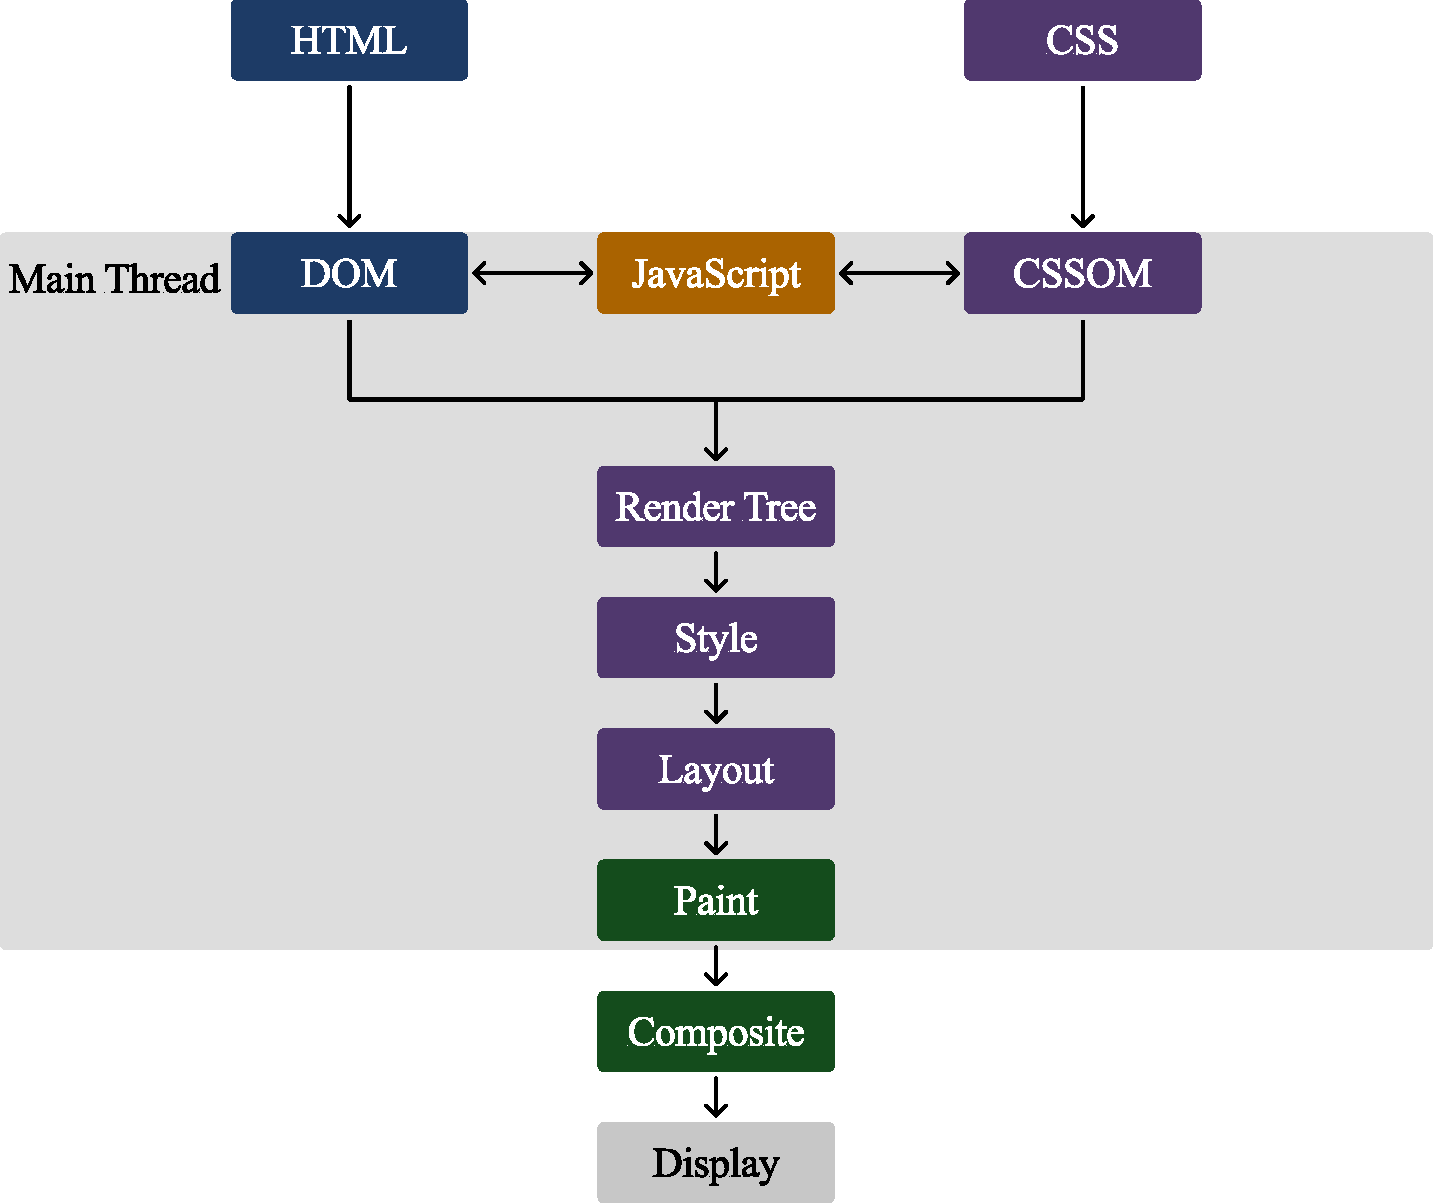
\includegraphics[width=0.8\textwidth,keepaspectratio]{bilder/rendering-pipeline.pdf}
	\caption[Phasenmodell des Critical Rendering Paths]{Phasenmodell des Critical Rendering Paths zur Verdeutlichung der Main-Thread-Auslastung (Eigene Darstellung in Anlehnung an \cite{web-dev-critical-path-2023}).}
	\label{fig:rendering-pipeline}
\end{figure}

\subsubsection{DOM als zentrale Repräsentation der UI}
\label{sss:dom}

Das DOM stellt die Inhalte hierarchisch in Form eines Baumes dar. Durch diese programmierbare Schnittstelle erhalten Skriptsprachen Zugriff auf die Objekte des Dokuments und können so Struktur und Inhalte flexibel verändern. Eltern-Kind-Beziehungen im DOM-Baum übersetzen die Verschachtelung des Quelltexts und bilden so die Grundlage für die Interaktivität moderner Webanwendungen \cite{mdn_dom_2026}. Jede dieser Änderungen am DOM kann dabei Rendering-Prozesse auslösen (vgl.\ \cref{sss:reflow-repaint-composite}).

\subsubsection{Sichtbarkeit im Render Tree und Layout-Abhängigkeiten}
\label{sss:visibility-render-tree-layout}

Bei der Modellbildung im Render Tree ist insbesondere zwischen \texttt{display: none} (nicht im Render Tree enthalten) und \texttt{visibility: hidden} (Elemente sind im Render Tree enthalten, belegen Layoutplatz, bleiben jedoch unsichtbar) zu unterscheiden \cite{web.dev_rclp_2014}. 
\Cref{fig:dom_cssom_render_tree} veranschaulicht diesen zentralen Unterschied zwischen logischer Struktur und visueller Repräsentation im Rahmen des Critical Rendering Paths. Während des Layout-Schritts wandelt der Browser die Knoten des Render Trees in konkrete Koordinaten um und bestimmt für jedes sichtbare Element innerhalb des Viewports, welche Ausmaße und Positionen es im Box-Modell einnimmt \cite{web.dev_rclp_2014}.
\begin{figure}[htb]
	\centering
	\narrowfig[0.7]{bilder/dom.pdf}
	\caption[Strukturelle Gegenüberstellung von DOM, CSSOM und Render Tree]{Strukturelle Gegenüberstellung von DOM, CSSOM und resultierendem Render Tree zur Veranschaulichung layoutrelevanter CSS-Eigenschaften. (Eigene Darstellung in Anlehnung an \cite{web.dev_rclp_2014}).}
	\label{fig:dom_cssom_render_tree}
\end{figure}

\subsubsection{Reflow, Repaint und Compositing: Performance-Kosten im Detail}
\label{sss:reflow-repaint-composite}

Je nach Art einer visuellen Änderung durchläuft der Browser die Rendering-Pipeline laut \cite{web.dev_rendering_2023} in drei unterschiedlichen Szenarien, die sich in ihrem Rechenaufwand stark unterscheiden. Eine Layout-Neuberechnung (Reflow) tritt auf, wenn sich geometrisch relevante Eigenschaften eines Elements ändern und der Browser dadurch die betroffenen und abhängigen Elemente im Layout erneut berechnen muss. Da Änderungen an einzelnen Elementen Auswirkungen auf die gesamte Hierarchie haben können, ist dieser Schritt besonders rechenintensiv. Handelt es sich um rein visuelle Anpassungen (z. B. Farbwechsel), führen diese lediglich zu einem Repaint, bei dem der Browser die betroffenen Pixelbereiche neu füllt, ohne die Geometrie erneut zu berechnen. Den effizientesten Weg stellt das Compositing dar, bei dem der Browser ausschließlich existierende Bildebenen (Layers) neu anordnet. Da dies oft auf einem eigenen Thread erfolgt, laufen insbesondere Animationen auf dieser Stufe besonders flüssig. Eine besondere Leistungsproblematik entsteht durch das sogenannte \textit{Layout Thrashing} \cite{web.dev_layoutthrashing_2025}. Dieses tritt auf, wenn JavaScript-Code Layout-Informationen abfragt (z. B. via \texttt{offsetWidth}), nachdem zuvor Stile verändert wurden \cite{web.dev_layoutthrashing_2025}. Da der Browser für die Abfrage einen aktuellen Wert liefern muss, erzwingt er eine sofortige, synchrone Neuberechnung (\textit{forced synchronous layout}), was zu einer ineffizienten Nutzung des Main Threads führt \cite{web.dev_layoutthrashing_2025}.

\subsection{Herausforderungen durch hochfrequente Updates (Main-Thread-Blocking)}
\label{ss:main-thread-blocking}

\subsubsection{Frame-Budget und Main-Thread-Überlastung}
\label{sss:frame-budget}

Damit eine Benutzeroberfläche flüssig wirkt, orientieren sich Browser nach \cite{web.dev_rendering_2023} an einer Bildwiederholrate von etwa 60 Bildern pro Sekunde. Daraus ergibt sich ein Zeitfenster von
\begin{equation}
	t_{\text{Frame}} = \frac{1000\,\mathrm{ms}}{60} \approx 16{,}7\,\mathrm{ms}
\end{equation}
pro Frame.
In der Praxis ist dieses Zeitfenster sogar noch knapper, da der Browser einen Teil dieser Zeit für interne Prozesse beansprucht. Letztlich verbleiben für die eigentliche Anwendungslogik oft nur etwa 10 ms. Innerhalb dieser kurzen Zeitspanne durchläuft der Browser die Rendering-Pipeline, die je nach Art der Änderung Prozesse wie die JavaScript-Ausführung, die Stil- und Layoutberechnung sowie das abschließende Painting und Compositing umfasst. Da diese Verarbeitungsschritte überwiegend sequenziell auf dem Main Thread ablaufen, führt jede Verzögerung innerhalb eines Einzelschritts zu einer Blockade des gesamten Renderprozesses \cite{mdn_mthread_2025}. Ergänzend definiert die Long Tasks API des World Wide Web Consortium (W3C) eine \qty{50}{ms}-Schwelle zur Identifikation blockierender Prozesse \cite{w3c_longtasks_2026}. Eine Aufgabe im Main Thread gilt als \textit{Long Task}, sobald ihre ununterbrochene Ausführungsdauer diesen Wert übersteigt.

\subsubsection{Auswirkungen auf Responsiveness und Benutzererfahrung}
\label{sss:user-expirience}

Ein häufiges Problem ist \textit{Input Delay}: Dabei verarbeitet der Browser Benutzereingaben wie Klicks oder Tastatureingaben nicht sofort, sondern erst nach Abschluss laufender Aufgaben, was zu einer spürbaren Verzögerung zwischen Eingabe und visueller Rückmeldung führt \cite{web.dev_inp_2025, w3c_longtasks_2026}. Als Maß für die Bewertung der Responsivität über die gesamte Besuchsdauer hinweg dient die Kennzahl INP (ausführliche Definition in \cref{ss:inp}). Ein weiteres Phänomen ist das sogenannte Jank \cite{web.dev_rendering_2023}. Dieses entsteht immer dann, wenn die Berechnung eines Frames länger dauert als das in \cref{sss:frame-budget} definierte Zeitfenster. Da der Browser in diesem Fall Frames überspringen muss, wirken Bewegungsabläufe wie Scrollen oder Animationen für den Nutzer stockend.

\subsubsection{Bedeutung für moderne UI-Frameworks (Synthese)}
\label{sss:ui-frameworks-synthesis}

Die in der Rendering-Pipeline entstehenden Kosten, insbesondere durch Layout- und Paint-Vorgänge (Reflows/Repaints), bilden die Grundlage für die Architektur moderner UI-Frameworks. Ziel dieser Frameworks ist es, die Anzahl direkter Eingriffe in das DOM zu minimieren. Anstatt jede Änderung sofort umzusetzen, bündelt das Framework Aktualisierungen. So ist sichergestellt, dass der Browser nur die tatsächlich veränderten Bereiche neu berechnen muss \cite{kumar-fluentreact-2024}. In der Praxis lassen sich dabei zwei unterschiedliche Strategien unterscheiden: Bibliotheken mit Virtual-DOM-Ansatz und compilerbasierte Frameworks. Diese grundlegenden Herangehensweisen werden in den folgenden Abschnitten detailliert analysiert.

\section{Architektur von React}
\label{s:react}

Dieser Abschnitt erläutert, wie React durch ein Virtual DOM (VDOM), Reconciliation und ergänzende Mechanismen diese Performance-Kosten adressiert.

\subsection{Virtual DOM und Reconciliation}
\label{ss:vdom}

Das VDOM ist eine Zwischenschicht im Speicher, die die Benutzeroberfläche mittels JavaScript-Objekten (React-Elementen) nachbildet. Wenn sich der Zustand (State) ändert, generiert React eine neue, virtuelle Darstellung des betroffenen React-Elementbaums. Durch das Bündeln mehrerer Änderungen (Batching) gibt React diese gesammelt an das reale DOM weiter, um die Anzahl teurer Layout-Neuberechnungen im Browser zu reduzieren \cite{kumar-fluentreact-2024}. Um die notwendigen Aktualisierungen zu identifizieren, nutzt React den Prozess der Reconciliation. Ein zentraler Bestandteil dieses Prozesses ist der Diffing-Algorithmus, ein rekursives Verfahren zum Vergleich der virtuellen Baumstrukturen. Während der Vergleich zweier beliebiger Baumstrukturen theoretisch eine Komplexität von $O(n^3)$ aufweist, reduziert React diesen Aufwand durch heuristische Annahmen (z. B. Elementtypen und Keys) in der Praxis auf annähernd $O(n)$ \cite{react_reconcillation_2024}. Da Zustandsänderungen standardmäßig Re-Renders entlang der nachgelagerten Teilbäume auslösen, steigt der Rechenaufwand dennoch direkt mit der Tiefe und Breite der betroffenen Komponentenstruktur \cite{kumar-fluentreact-2024}.


\subsection{Der React Compiler (ab React 19): Automatisierte Memoisierung vs. manuelles Opt-in}
\label{ss:react-compiler}

\subsubsection{Funktionsweise des React Compilers}
\label{sss:react-compiler}

Um unnötige Re-Renders zu vermeiden, mussten Entwickler bisher manuell mittels \texttt{React.memo} oder Hooks wie \texttt{useMemo} und \texttt{useCallback} memoisieren \cite{kumar-fluentreact-2024}. Diese Form der manuellen Memoisierung ist jedoch fehleranfällig und erhöht den kognitiven Aufwand während der Entwicklung \cite{react_introduction}. Der React Compiler verlagert diese Aufgaben in den Build-Prozess. Er untersucht den Code statisch mittels einer internen Zwischendarstellung (Intermediate Representation), analysiert den Datenfluss und fügt automatisch Optimierungen hinzu, die eine stabile Referenzgleichheit gewährleisten \cite{react_compiler_2025}. Im Gegensatz zu Svelte, welches Komponenten in DOM-nahen Code umwandelt, optimiert der React Compiler lediglich bestehende Komponenten durch intelligentes Caching, ohne das Laufzeitmodell grundlegend zu verändern \cite{kumar-fluentreact-2024}.


\subsubsection{Potenziale und Grenzen im Kontext der Skalierung}
\label{sss:potentials-and-limitations}

Die Automatisierung reduziert den Umfang an Boilerplate-Code und entlastet Entwickler von der Pflege von Abhängigkeitslisten (Dependency-Arrays) \cite{react_introduction}. Da der Compiler ausschließlich bestehende Komponenten memoisiert, bleiben die grundlegenden architekturbedingten Kosten von VDOM-Diffing und Reconciliation (\cref{ss:vdom}) sowie die damit verbundenen Heap-Allokationen jedoch bestehen \cite{kumar-fluentreact-2024, thedatascientist_vdom}.

\subsection{Fiber-Engine: Scheduling und Rendering}
\label{ss:fiber-engine}

Um synchron-blockierende Updates im Komponentenbaum zu verhindern, überarbeitete React die interne Verarbeitung grundlegend \cite{github-reactfiber-2016}.

\subsubsection{Aufbau der Fiber-Architektur}
\label{sss:fiber-engine-structure}

Fiber stellt eine interne Struktur zur Organisation und Planung von Arbeitsschritten (Scheduling) dar, wobei ein einzelner Fiber die kleinste unterbrechbare Arbeitseinheit repräsentiert \cite{github-reactfiber-2016}. Hierzu überführt Fiber den UI-Baum in eine mit expliziten Zeigern (Kind, Geschwister, Elternteil) verkettete Struktur, wodurch React laufende Prozesse bei Bedarf verwerfen, unterbrechen, den aktuellen Stand zwischenspeichern und die Ausführung ohne Kontextverlust später fortsetzen kann. Da Fiber den Call Stack lediglich nachbildet, bleibt die $O(n)$-Komplexität beim Diffing unverändert \cite{github-reactfiber-2016, react_reconcillation_2024}. Um diese Berechnungen ohne sofortige Auswirkung auf die Anzeige durchzuführen, nutzt die Architektur das Prinzip des \textit{Double Buffering}, bei dem ein im Hintergrund bearbeiteter Baum (\textit{work-in-progress}) erst nach Abschluss den sichtbaren Baum (\textit{current}) ersetzt, wie in \cref{fig:react_fiber_trees} veranschaulicht \cite{medium_fiber-2024}. Während Fiber-Knoten persistent sind und wiederverwendet werden, entstehen React-Elemente bei jedem Render-Vorgang neu \cite{dev_fiber-2018}. Die JavaScript-Engine V8 verwaltet diese kurzlebigen Objekte effizient im sogenannten \textit{jungen Speicherbereich} (Young Generation). Um die Auswirkungen auf den Main Thread bei der regelmäßigen Garbage Collection (GC) so gering wie möglich zu halten, lagert V8 diese Prozesse teilweise auf parallele Hilfs-Threads aus \cite{v8.dev_fiber-2019}. Wenn jedoch eine sehr hohe Anzahl an UI-Elementen gleichzeitig gerendert wird, summieren sich diese kleinen Rechen- und Speicheraufwände. Dadurch entsteht ein spürbarer Overhead, was die Skalierbarkeit im Vergleich zu Ansätzen ohne VDOM einschränken kann \cite{svelte_vdom-2018}.
\begin{figure}[H]
	\centering
	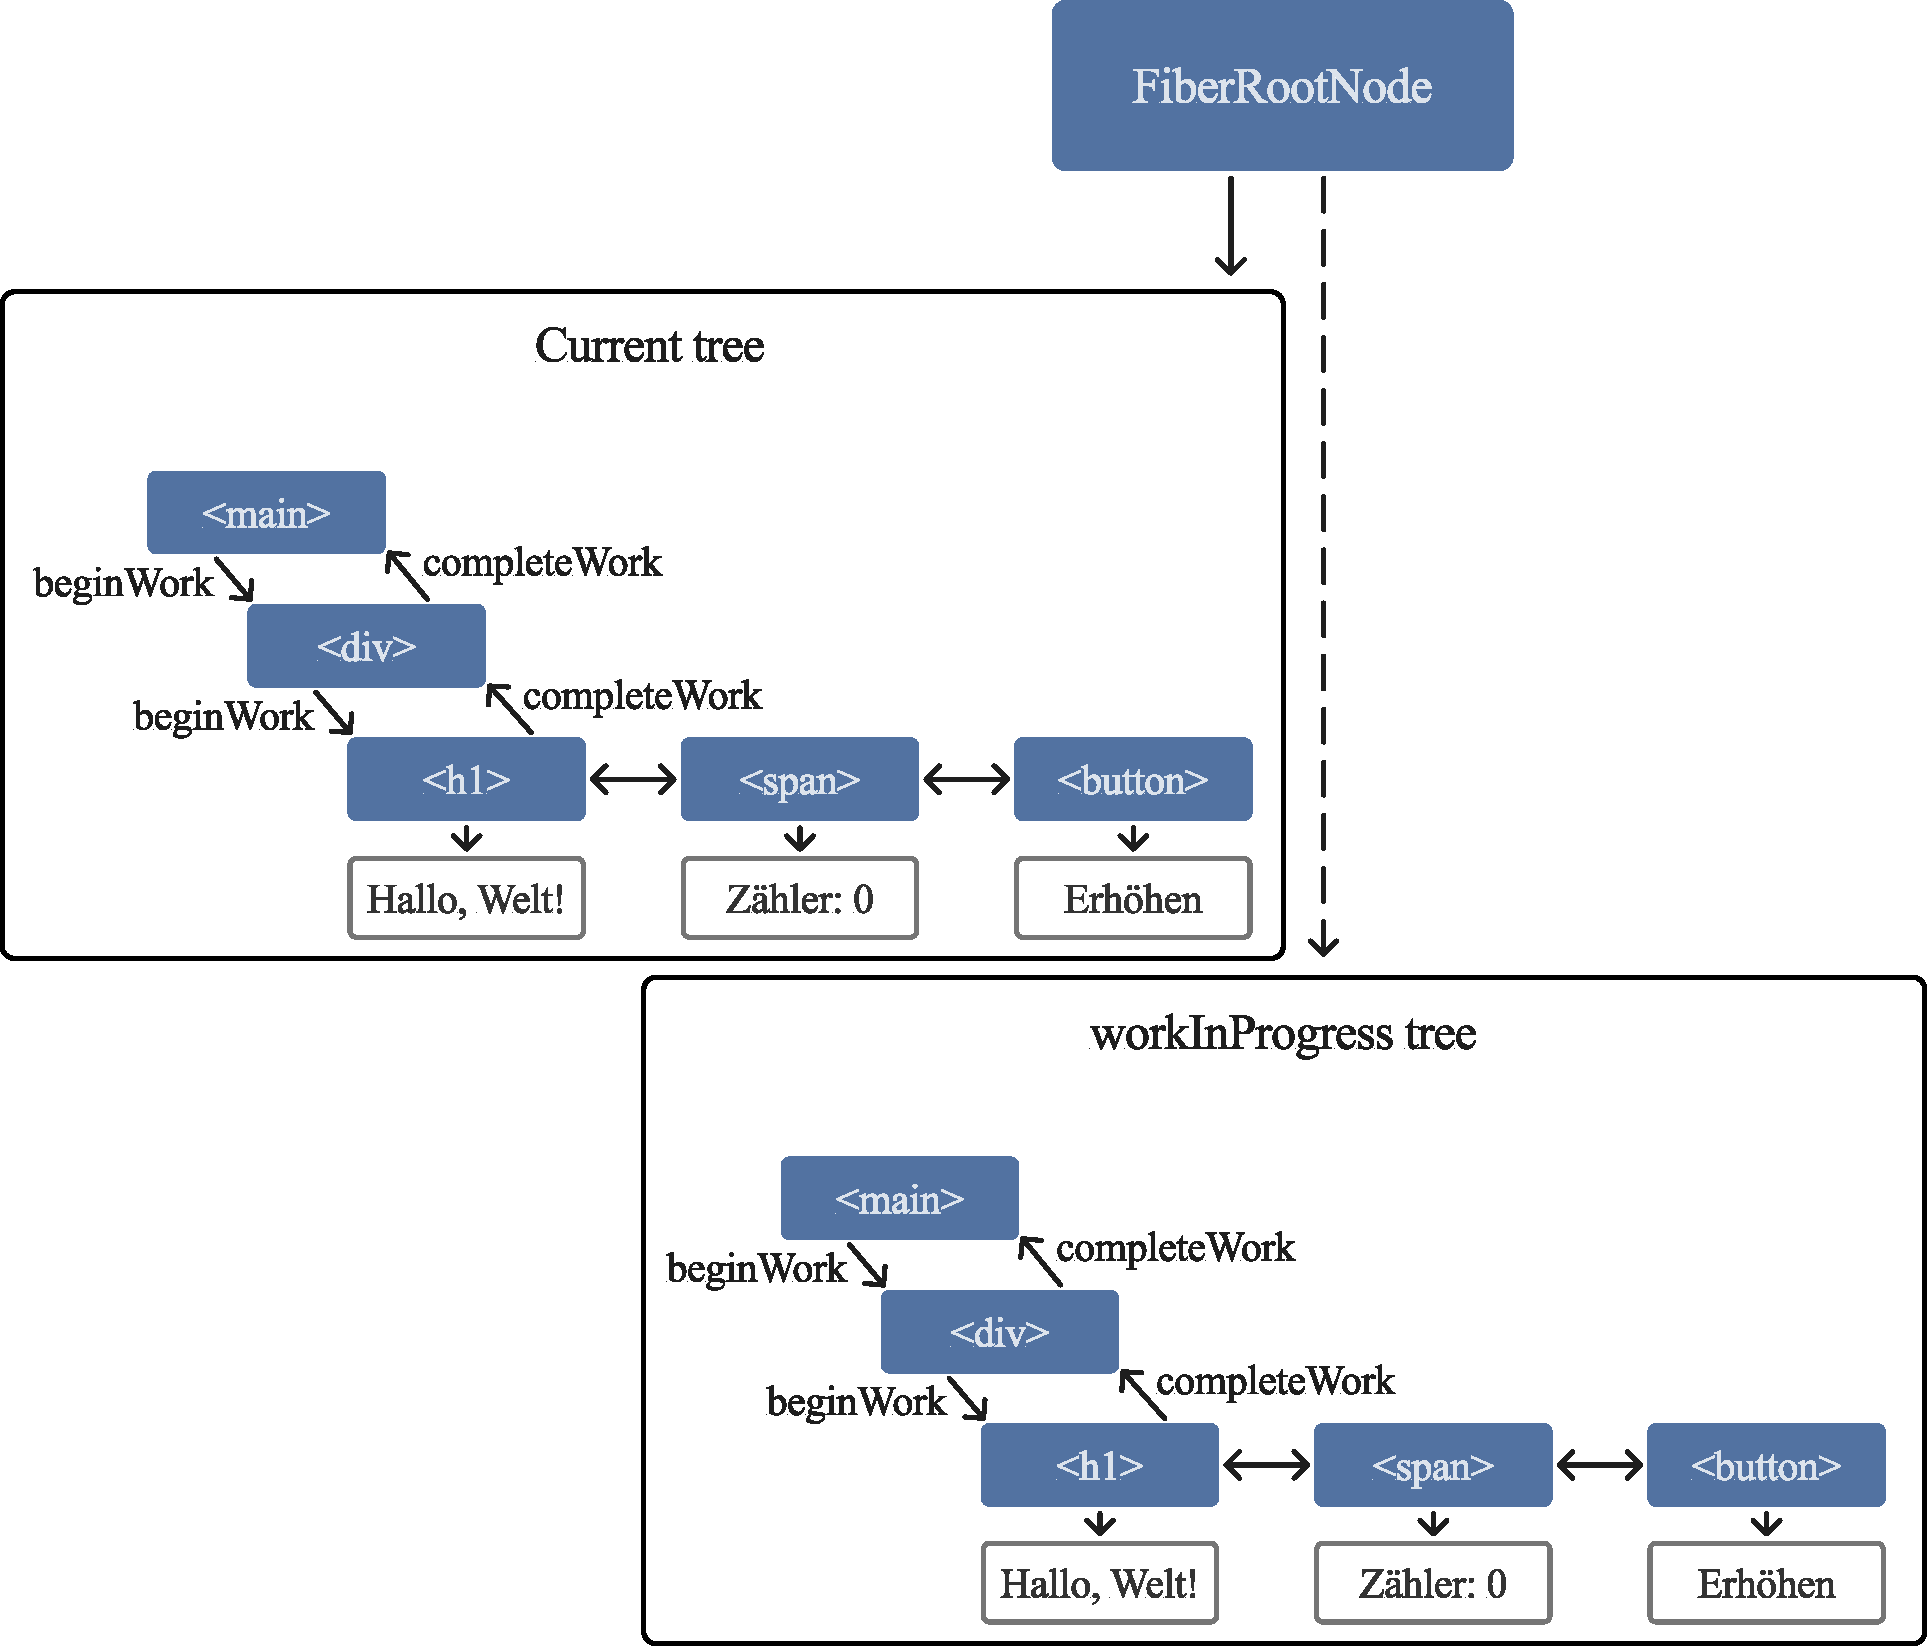
\includegraphics[width=0.8\textwidth,height=0.35\textheight,keepaspectratio]{bilder/fiber_double_buffering.pdf}
	\caption[Architekturmodell der React Fiber-Engine]{Architekturmodell der React Fiber-Engine: Double Buffering und Umschalten des FiberRootNode auf den Work-in-Progress Tree während der Commit-Phase. (Eigene Darstellung in Anlehnung an \cite{kumar-fluentreact-2024}).}
	\label{fig:react_fiber_trees}
\end{figure}

\subsubsection{Scheduling und Priorisierung von Updates}
\label{sss:scheduling-priotising-of-updates}

Um den Main Thread nicht zu blockieren, zerlegt das System anstehende Aufgaben per \textit{Time Slicing} in kleinere Arbeitsschritte. Über Render Lanes (Bitmasken) priorisiert das System Aufgaben nach Dringlichkeit: Nutzerinteraktionen (z. B. Klicks) erhalten stets Vorrang, Hintergrundprozesse laufen nachrangig \cite{kumar-fluentreact-2024}. Der Scheduler nutzt einen kooperativen Yielding-Ansatz: Nach der Bearbeitung einzelner Fiber-Knoten prüft der Scheduler, ob ein internes Zeitbudget (~5 ms) überschritten ist; ist dies der Fall, gibt er die Kontrolle an den Browser zurück \cite{dev_fiber-2025}. Übersteigt das Aufkommen an Updates die Kapazität des Schedulers, führt dieser Verarbeitungsstau zu verzögerten Render-Vorgängen und dazu, dass das Zeitfenster pro Frame trotz Priorisierung nicht mehr eingehalten werden kann \cite{sitepoint_fiber-2026}. Neben der Kompensation des Reconciliation-Overheads erfüllt das \textit{Time Slicing} eine weitere Funktion: Der kooperative Yielding-Ansatz begrenzt die maximale ununterbrochene Blockierungsdauer des Main Threads \cite{github-reactfiber-2016, react_concurrentrendering-2022}. Im Gegensatz dazu verfügt Svelte über kein integriertes \textit{Time Slicing} \cite{github-reactfiber-2016, medium-microtasks-2021}. Stattdessen fasst das Effect-Batching (\cref{sss:microtasks}) ausstehende Zustandsänderungen zusammen und arbeitet sie gebündelt im darauffolgenden Microtask ab \cite{svelte-effect}. Eine Verteilung noch ausstehender Arbeit auf nachfolgende Frames ist in dieser Architektur nicht vorgesehen \cite{medium-microtasks-2021, github-reactfiber-2016}.


\subsubsection{Concurrent Rendering}
\label{sss:concurrent-rendering}

Aufbauend auf der Fiber-Struktur und der Priorisierung ermöglicht Concurrent Rendering die Vorbereitung neuer UI-Zustände im Hintergrund, ohne die sichtbare Oberfläche direkt zu verändern \cite{react_concurrentrendering-2022}. Für eine hohe Reaktionsfähigkeit gliedert sich der Ablauf in zwei Phasen \cite{medium_fiber-2018}:
\begin{enumerate}
	\item \textbf{Render-Phase (asynchron):} Das System identifiziert mittels Diffing die erforderlichen Änderungen. Dieser Prozess ist unterbrechbar.
	\item \textbf{Commit-Phase (synchron):} React nimmt die Änderungen am realen DOM vor. Dieser Schritt ist stets synchron und nicht unterbrechbar \cite{medium_fiber-2018}.
\end{enumerate}
Die Dauer der Commit-Phase hängt direkt von der Anzahl der zu aktualisierenden DOM-Elemente ab \cite{kumar-fluentreact-2024}. Bei hoher UI-Dichte kann diese Phase das Frame-Budget ununterbrechbar belegen, was zu Jank führt und die Interaktionslatenz (INP) unmittelbar verlängert \cite{web.dev_fiber_2025}.

\section{Architektur von Svelte}
\label{s:svelte}

Während der in \cref{s:react} untersuchte Ansatz von React stark auf eine komplexe Laufzeitumgebung und den Vergleich eines VDOM setzt, wählt Svelte einen anderen Ansatz. Statt Änderungen erst im Browser zur Laufzeit zu berechnen, verlagert Svelte diese Arbeit in den Build-Prozess \cite{github-svelte_arch-2017}.

\subsection{Compilerbasierter Ansatz}
\label{ss:svelte-compiler}

Beim Build-Prozess überführt der Compiler den deklarativen Code in einen abstrakten Syntaxbaum (AST) und generiert daraus spezifische Code-Fragmente für das Erstellen, Aktualisieren und Entfernen einzelner DOM-Knoten \cite{github-svelte_arch-2017, svelte_vdom-2018}. Welche dieser Fragmente bei einer Datenänderungen ausgeführt werden, bestimmt in Svelte 5 die Signal-Architektur zur Laufzeit (vgl.\ \cref{ss:svelte-reactivity}), sodass das System ausschließlich die unmittelbar betroffenen Operationen ausführt. Durch den Verzicht auf ein VDOM und die damit verbundenen Reconciliation-Prozesse reduziert sich die Rechenlast auf dem Main Thread sowie der Speicherbedarf erheblich \cite{svelte_vdom-2018, ollila-rendering_performance-2022}. Dies führt zu weniger Objektzuweisungen im Heap und entlastet die Garbage Collection, wodurch pro Frame mehr Zeit für eine flüssige Darstellung zur Verfügung steht \cite{svelte-reactivity-2019}.

\subsection{Reaktivität und Update-Mechanismen}
\label{ss:svelte-reactivity}

Im Gegensatz zum klassischen Svelte-Compiler, der Abhängigkeiten ausschließlich statisch zur Kompilierzeit ermittelt hat, setzt Svelte 5 auf das Modell der Signals \cite{svelte_runes_2023}. Entwickler nutzen hierzu spezifische Compiler-Anweisungen, sogenannte Runes (z. B. \texttt{\$state} und \texttt{\$derived}). Während Runes die syntaktische Schnittstelle bilden, identifizieren Signals zur Laufzeit automatisch die Abhängigkeiten zwischen den Werten \cite{svelte_migration}.

\subsubsection{Mechanismus der feingranularen Reaktivität}
\label{sss:finegraned-reactivity}

Die Signal-Architektur ermöglicht eine feingranulare Reaktivität \cite{svelte_runes_2023, balasubramanian-signal-2025}, bei der die gesamte Verarbeitung, von der Erkennung einer Zustandsänderung über die Auswertung der betroffenen Abhängigkeiten bis zur gezielten DOM-Aktualisierung, auf die jeweils betroffenen Knoten begrenzt bleibt \cite{svelte_runes_2023, balasubramanian-signal-2025}. Zustandsänderungen lassen sich so auch bei Arrays aus primitiven Datentypen genau nachverfolgen, ohne die ursprüngliche Datenstruktur anzupassen \cite{svelte_fine-grained_reactivity-2023}. Im Vergleich zur Reconciliation in React, die oft mehrere Abgleichschritte über Teilbäume erfordert, reduziert dieser Ansatz den Aufwand pro Interaktion meist auf eine einzige gezielte Operation \cite{putra-performance-2025}.

\subsubsection{Speichermodell und Overhead von Runes}
\label{sss:runes-overhead}

Intern bildet Svelte Signals als einfache JavaScript-Objekte (POJOs) ab, die sowohl bei der Erstellung als auch beim Zugriff deutlich ressourcensparender sind als komplexe Klasseninstanzen \cite{github-svelte_bench_13277-2024}. Im Unterschied zu den baumartigen Fiber-Strukturen von React (\cref{sss:fiber-engine-structure}) schafft dieser compilerbasierte Ansatz die strukturellen Voraussetzungen für eine effizientere Skalierung, insbesondere bei großen Mengen an UI-Elementen \cite{putra-performance-2025}. Der Overhead pro Signal ist zwar minimal, doch bei jedem Update muss das System jede reaktive Abhängigkeit einzeln auswerten (\cref{sss:finegraned-reactivity}). Bei gleichzeitiger Aktualisierung aller $n$ Elemente wächst der Gesamtaufwand ebenfalls mit $O(n)$ — dieselbe Komplexitätsklasse wie die Reconciliation in React (\cref{ss:vdom}), allerdings mit einem geringeren Aufwand pro Element. Ab welchem $n$ dieser Unterschied praktisch vernachlässigbar wird, lässt sich theoretisch nicht bestimmen.

\subsubsection{Vermeidung von Render-Flaschenhälsen}
\label{sss:rendering-bottleneck}

Die feingranulare Signal-Architektur reduziert die CPU-Belastung deutlich, da die Implementierung gezielt darauf ausgelegt ist, ineffiziente Ausführungen in der JavaScript-Engine (V8) zu vermeiden und besonders häufig genutzte Codebereiche (\textit{Hot Paths}) zu optimieren \cite{github-svelte_bench_13277-2024}. In Kombination mit sehr schnellen Ausführungszeiten und nur minimalen Eingriffen ins DOM sinkt dadurch die Wahrscheinlichkeit für Long Tasks (\cref{sss:frame-budget}). Daraus lässt sich ableiten, dass Svelte selbst unter hoher Last kein aufwendiges Laufzeit-Scheduling wie etwa das Time Slicing in React benötigt, da die einzelnen Verarbeitungsschritte von vornherein klein und effizient gehalten sind.


\subsection{Effizienz der imperativen DOM-Updates}
\label{ss:svelte-efficiency}

\subsubsection{Ausführung imperativer DOM-Befehle}
\label{sss:running-dom-commands}

Zur Erstellung von DOM-Strukturen nutzt der Compiler Verfahren wie das Klonen von \texttt{<template>}-Elementen oder den schrittweisen programmatischen Aufbau \cite{svelte-compiler}. Die Darstellung von Template-Ausdrücken und deren Logik basiert intern auf Effekten. Diese sorgen automatisiert dafür, dass Datenänderungen unmittelbar zu einer Anpassung des DOM führen. Für Spezialfälle, in denen bestimmte Operationen noch vor der eigentlichen DOM-Aktualisierung erfolgen müssen, stellt Svelte zusätzlich \texttt{effect.pre} bereit \cite{svelte-effect}.


\subsubsection{Effect-Batching und Microtasks}
\label{sss:microtasks}

Ändert sich der Zustand in einer Svelte-Anwendung, passt Svelte das DOM nicht sofort nach jeder einzelnen Änderung an \cite{medium-microtasks-2021}. Stattdessen bündelt Svelte Zustandsänderungen per Microtask: Das Framework fasst mehrere gleichzeitige Änderungen zusammen, bevor DOM-Anpassungen und Effects folgen \cite{svelte-effect}. Dadurch lässt sich das in \cref{sss:reflow-repaint-composite} beschriebene Layout Thrashing wirksam vermeiden. 


\subsubsection{Theoretische Grenzen (JS-zu-DOM-Flaschenhals)}
\label{sss:theoretical-limitations}

Trotz dieser Optimierungen bleibt Svelte an die grundlegenden Grenzen der Browser-Architektur gebunden. Zwar sind die JavaScript-Engine und die Rendering-Engine eigenständige Komponenten, sie arbeiten jedoch über klar definierte Schnittstellen wie das DOM und die Web-IDL-Bindings eng zusammen \cite{mdn-javascript_engine}. Jeder Zugriff auf diese Verbindung zwischen JavaScript und der Rendering-Schicht bringt dabei einen systembedingten Overhead mit sich \cite{chromium-blink_faq}. Bei einer extremen kombinierten Last aus UI-Dichte und Update-Frequenz können daher auch unter Svelte blockierende Long Tasks und Interaktionslatenzen auftreten, da sich die Kosten für wiederholte DOM-Zugriffe summieren (\cref{sss:frame-budget}).

\section{Vergleichbare Metriken und Performancebegriffe}
\label{s:metrics}

\subsection{Interaktionslatenz und Antwortverhalten (INP)}
\label{ss:inp}

\subsubsection{Definition und Phasen der Metrik}
Die Metrik Interaction to Next Paint (INP) misst, wie schnell eine Webseite auf Nutzerinteraktionen über die gesamte Nutzungsdauer hinweg reagiert \cite{web.dev_inp_2025}. Die technische Zusammensetzung der Metrik sowie die zeitliche Abfolge der einzelnen Phasen sind in \cref{fig:inp-phases} dargestellt. Aus technischer Sicht lässt sich dieser Messwert in drei Phasen unterteilen \cite{web.dev_inp_2025}:
\begin{itemize}
	\item \textbf{Input Delay (Eingabeverzögerung):} Zeitspanne vom Beginn der Nutzerinteraktion bis zur Verarbeitung des ersten Event-Handlers, verursacht durch Main-Thread-Blockaden (vgl. \cref{ss:main-thread-blocking}).
	\item \textbf{Processing Time (Verarbeitungsdauer):} Hierbei handelt es sich um die Zeit zur vollständigen Ausführung aller Callbacks der Event-Handler und der damit verbundenen Framework-Logik.
	\item \textbf{Presentation Delay (Darstellungsverzögerung):} Diese Phase misst die Zeit nach Abschluss der Skriptausführung bis zu dem Punkt, in dem der Browser die Änderungen sichtbar auf dem Bildschirm darstellt.
\end{itemize}
Google definiert auf Basis dieser Metrik drei Leistungskategorien: INP-Werte bis einschließlich $200\,\text{ms}$ gelten als \textit{Good}; Werte zwischen $200\,\text{ms}$ und $500\,\text{ms}$ als \textit{Needs Improvement}; Werte oberhalb von $500\,\text{ms}$ als \textit{Poor} \cite{web.dev_inp_2025}.
\begin{figure}[H]
	\centering
	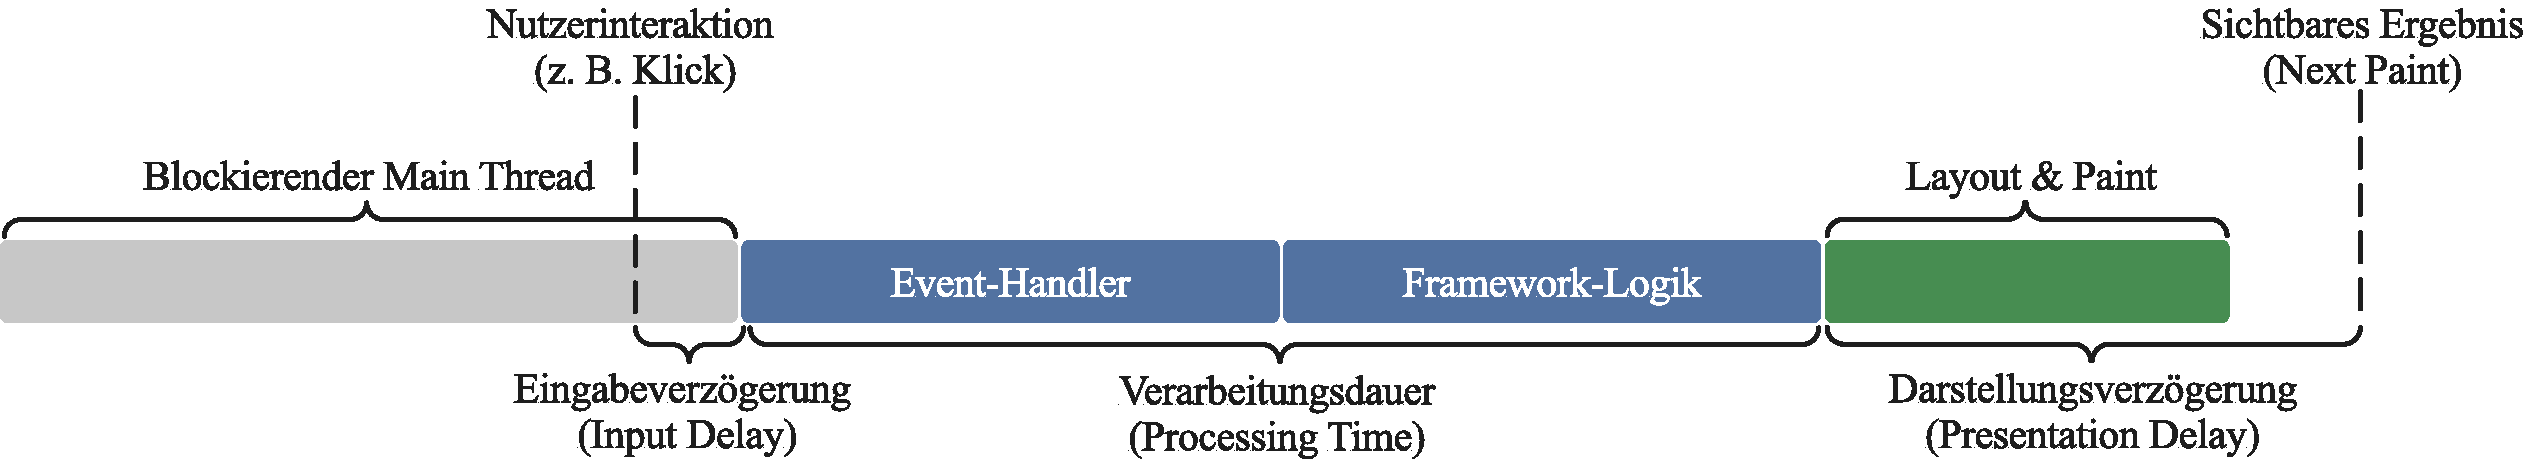
\includegraphics{bilder/inp_phasenmodell.pdf}
	\caption[Zeitliches Phasenmodell der INP-Metrik]{Zeitliches Phasenmodell der Metrik Interaction to Next Paint (INP) vom Auslösen des Events bis zum Rendering. (Eigene Darstellung in Anlehnung an \cite{web.dev_inp_2025}).}
	\label{fig:inp-phases}
\end{figure}

\subsubsection{Messung aller Interaktionen und Abgrenzung zu FID}
Im Gegensatz zum \textit{First Input Delay} (FID), welcher nur die erste Interaktion erfasst, bewertet INP die Stabilität der Performance während der gesamten Sitzung. Der finale INP-Wert entspricht in der Regel der Interaktion mit der höchsten Gesamtverzögerung. Damit einzelne Ausreißer das Ergebnis nicht verzerren, ignoriert die Metrik bei jeweils 50 Interaktionen den höchsten Wert. Auf diese Weise entsteht ein realistischeres Bild der tatsächlichen, stabilen Performance \cite{web.dev_inp_2025}.

\subsubsection{Relevanz für die Messung der UI-Skalierung}
INP dient als zentrale Metrik, um den in \cref{sss:tipping-point} beschriebenen Tipping Point empirisch zu identifizieren. Sie macht messbar, ab welcher kombinierten Last aus UI-Dichte und Update-Frequenz die \textit{Processing Time} oder das \textit{Presentation Delay} das verfügbare Frame-Budget überschreitet und zu spürbaren Verzögerungen führt.


\subsection{Analyse der Speichereffizienz (Heap-Snapshots)}
\label{ss:memory-efficiency}

\subsubsection{Funktionsweise von Heap-Snapshots}
Ein Heap-Snapshot stellt eine detaillierte Momentaufnahme des Objektgraphen innerhalb des Speichers der JavaScript-Laufzeitumgebung dar \cite{chrome-memory-terminology-2024}. Er dient dazu, die Speicherverteilung zu untersuchen, mögliche Speicherlecks zu erkennen oder Objekte zu identifizieren, die übermäßig viele Ressourcen im System beanspruchen \cite{chrome-heap-snapshots-2024}.

\subsubsection{Shallow Size vs. Retained Size}
Zur genauen Messung des Speicherverbrauchs sind zwei zentrale Metriken zu unterscheiden: Die \textit{Shallow Size} umfasst den Speicherplatz, den ein Objekt für sich selbst beansprucht, ohne dabei den Speicher der referenzierten Objekte einzubeziehen.
Die \textit{Retained Size} hingegen beschreibt, wie viel Speicher freigegeben werden kann, wenn ein bestimmtes Objekt aus dem Speicher entfernt wird. Sie umfasst dabei nicht nur das Objekt selbst, sondern auch alle abhängigen Elemente, die ausschließlich über dieses Objekt referenziert wurden und nach dessen Entfernung keine Verbindung mehr zu den Garbage-Collector-Wurzeln haben \cite{chrome-memory-terminology-2024}.

\subsubsection{Analyse des Objekt-Graphen: Distance und Dominators}

Die \textit{Distance} gibt die Anzahl der Schritte von der Wurzel des Garbage Collectors (GC Root) zum Objekt an. Weisen Objekte gleichen Typs ungewöhnlich große Distanzen auf, deutet das oft auf komplexe und speicherintensive Referenzketten hin \cite{chrome-memory-terminology-2024}. Strukturell basiert die Retained Size im Wesentlichen auf dem Konzept der \textit{Dominators} (Dominatoren). Dabei gilt ein Objekt $d$ als Dominator eines anderen Objekts $n$, wenn jeder mögliche Pfad vom Root-Knoten zu $n$ zwangsläufig über $d$ führt \cite{bynens-lorenz-memory-profiling}. Innerhalb des Speicher-Graphen lassen sich Dominator-Beziehungen als Baumstruktur darstellen \cite{chrome-memory-terminology-2024}. Diese Struktur ist besonders wichtig für die Retained Size, da beim Entfernen eines Objekts auch alle davon abhängigen Objekte im zugehörigen Zweig für die Garbage Collection freigegeben werden. Diese baumartige Hierarchie sowie das Zusammenspiel der Metriken Distance, Shallow Size und Retained Size werden in \cref{fig:heap_dominator_tree} zusammenfassend visualisiert. Für den empirischen Framework-Vergleich ist die Retained Size die geeignetste Kennzahl, da sie den internen Framework-Overhead vom Anwendungszustand trennt. Die methodische Umsetzung dieser Messung erläutert \cref{ss:memory-measurement}.
\begin{figure}[H]
	\centering
	\narrowfig[0.7]{bilder/heap_dominator_tree.pdf}
	\caption[Modell eines Speicher-Graphen zur Darstellung der Retained Size]{Modell eines Speicher-Graphen zur Veranschaulichung der Dominator-Beziehungen sowie der Differenzierung zwischen Shallow und Retained Size. (Eigene Darstellung in Anlehnung an \cite{chrome-memory-terminology-2024}).}
	\label{fig:heap_dominator_tree}
\end{figure}

\subsection{Scripting- vs. Rendering-Zeit im Browser-Profil}
\label{ss:profiling-categories}

\subsubsection{Kategorien im Performance-Trace}
Werkzeuge wie das Chrome DevTools Performance-Panel visualisieren die Main-Thread-Auslastung in Kategorien \cite{chrome-performance-reference-2024}:

\begin{itemize}
	\item \textbf{Scripting (Gelb):} Diese Kategorie beschreibt die gesamte Zeit, die die JavaScript-Engine für das Parsen, Kompilieren und Ausführen von JavaScript-Code benötigt \cite{chrome-lighthouse-js-execution-2019, chrome-performance-reference-2024}.
	
	\item \textbf{Rendering (Lila):} Die \textit{Rendering-Zeit} umfasst alle Phasen, in denen der Browser nach Zustandsänderungen die Stile der Elemente neu berechnet (\textit{Recalculate Style}) und anschließend die Geometrie des Dokumentenbaums bestimmt (\textit{Layout}) \cite{chrome-performance-reference-2024}.
	
	\item \textbf{Painting:} Diese Phase beschreibt den Prozess, bei dem der Browser die grafischen Zeichenbefehle in Pixel umwandelt, bevor der Browser diese im nächsten Schritt final zur Bildschirmausgabe zusammensetzt \cite{chromium-frameviewer-howto}. 
\end{itemize}

\subsubsection{Bedeutung für die Tipping-Point-Analyse}

Die getrennte Analyse dieser Kategorien hilft dabei zu erkennen, wo Leistungsengpässe entstehen. Während die \textit{Scripting-Zeit} den internen Aufwand der Framework-Logik (z. B. Reconciliation oder Signal-Auswertung) widerspiegelt, zeigt die Rendering-Zeit die Last der Browser-Engine beim Umsetzen der DOM-Änderungen \cite{chrome-performance-reference-2024, chromium-frameviewer-howto}. Dies ist essenziell für die Untersuchung der theoretischen Skalierungsgrenzen (\cref{sss:theoretical-limitations}).


\section{Theoretische Vergleichsmodelle und Hypothesen}
\label{s:theoretical-models-and-hypotheses}

Dieses Kapitel überführt die architektonischen Merkmale aus \cref{s:react} und \cref{s:svelte} in ein vergleichendes Modell. Ziel ist es, die Auswirkungen von UI-Dichte ($n$) und Update-Frequenz ($f$) auf die Systemleistung theoretisch herzuleiten.

\subsection{Synthese der Abstraktionskosten}
\label{ss:abstraction-costs}

Der Vergleich zwischen dem VDOM-basierten Ansatz und der direkten DOM-Manipulation zeigt grundlegende Unterschiede in der Ressourcenallokation. Während der in \cref{ss:vdom} beschriebene Diffing-Prozess von React bei Zustandsänderungen einen algorithmischen CPU-Overhead zur Laufzeit verursacht, entfällt dieser Reconciliation-Overhead bei der Compiler-Architektur von Svelte (\cref{ss:svelte-compiler}) fast vollständig. Dies betrifft auch den Speicherbedarf: Durch den VDOM-Ansatz werden fortlaufend virtuelle Knoten erzeugt, wodurch die Belastung der Garbage Collection linear mit der Anzahl der Elemente $n$ ansteigt \cite{bai-millionjs-2023, github-reactfiber-2016}. Svelte umgeht diese Zwischenstrukturen und entlastet so die JavaScript-Laufzeitumgebung (\cref{ss:svelte-compiler}). Unabhängig davon sind beide Architekturen jedoch auf die native DOM-Schnittstelle angewiesen, was bei hoher Skalierung zu einem unvermeidbaren Flaschenhals im Main Thread führt (\cref{sss:theoretical-limitations}).

\subsection{Komplexität und Skalierung (n vs. f)}
\label{ss:update-complexity}

\subsubsection{Umfang der Neuberechnungen bei Zustandsänderungen} 

In der React-Architektur skaliert der Berechnungsaufwand bei Zustandsänderungen unabhängig von tatsächlichen DOM-Veränderungen direkt proportional zur Anzahl der Knoten im betroffenen Teilbaum (\cref{ss:vdom}). Im Gegensatz dazu entkoppelt das feingranulare Reaktivitätsmodell von Svelte (\cref{ss:svelte-reactivity}) den Aufwand von der Baumgröße. Da keine Diffing-Schritte über nicht betroffene Komponenten nötig sind, bestimmt sich die Ausführungszeit primär durch die Anzahl der tatsächlich veränderten Abhängigkeiten (\cref{sss:finegraned-reactivity}).

\subsubsection{Der Multiplikator-Effekt und der Tipping Point}
\label{sss:tipping-point}

Die Kombination aus hoher Frequenz $f$ und hoher Dichte $n$ führt zu einer gegenseitigen Verstärkung der Last. Da React bei jeder Änderung den entsprechenden Teilbaum erneut überprüft (\cref{ss:vdom}), kann die CPU-Auslastung bei hoher UI-Dichte und gleichzeitig hoher Aktualisierungsrate das Frame-Budget von 16,7 ms (\cref{sss:frame-budget}) vergleichsweise schnell ausschöpfen. Svelte begrenzt diesen Effekt durch direkte Operationen am relevanten Knoten (\cref{sss:finegraned-reactivity}). Aus den architektonischen Skalierungsunterschieden lässt sich ein theoretischer Tipping Point ableiten. Dieser bezeichnet den Übergang, an dem die aufsummierte Last den Main Thread durch Long Tasks blockiert (\cref{sss:frame-budget}). Bedingt durch baumgrößenabhängige Re-Render-Zyklen und die synchrone, nicht unterbrechbare Commit-Phase (\cref{sss:concurrent-rendering}) ist davon auszugehen, dass React diesen Punkt früher erreicht als Svelte. Bei vollständiger Aktualisierung aller $n$ Elemente pro Tick wächst auch der Aufwand der feingranularen Reaktivität linear mit $n$ (\cref{sss:runes-overhead}). Ab einem bestimmten Sättigungspunkt kann daher auch Svelte den Main Thread durch Long Tasks blockieren (\cref{sss:theoretical-limitations}). Da Sveltes Effect-Batching die gesamte Verarbeitung synchron innerhalb desselben Microtask-Zyklus abschließt (\cref{sss:microtasks}), während Reacts Time Slicing Arbeitsschritte über mehrere Frames verteilen kann (\cref{sss:scheduling-priotising-of-updates}), ist eine Umkehr der Tipping-Point-Rangfolge bei extremer kombinierter Last theoretisch nicht auszuschließen.


\subsection{Erwartetes Skalierungsverhalten}
\label{ss:expected-scaling}

Aus den in \cref{ss:update-complexity} beschriebenen Skalierungsunterschieden lässt sich erwarten, dass die Scripting-Zeit beider Frameworks unterschiedlich stark mit $n$ wächst. Die Reconciliation durchläuft dabei stets den gesamten betroffenen Teilbaum mit $O(n)$, unabhängig davon, wie viele Knoten sich tatsächlich verändert haben (\cref{ss:vdom}). Hinzu kommt der in \cref{sss:fiber-engine-structure} beschriebene GC-Overhead durch kurzlebige React-Elemente, der konzeptionell linear mit $n$ wächst (\cref{ss:abstraction-costs}). Svelte hingegen begrenzt den Scripting-Aufwand durch die feingranulare Reaktivität (\cref{sss:finegraned-reactivity}) auf die Auswertung der tatsächlich veränderten Abhängigkeiten. Da keine Diffing-Schritte über unveränderte Komponenten anfallen (\cref{ss:update-complexity}), ist davon auszugehen, dass der Aufwand nicht mit der Gesamtgröße des Komponentenbaums wächst, sondern mit der Anzahl der Änderungen. Auch wenn beide Architekturen bei vollständiger Aktualisierung mit $O(n)$ skalieren, ist der Aufwand pro Element bei Svelte theoretisch geringer, da der Abgleich des Komponentenbaums und die damit verbundenen Heap-Allokationen entfallen (\cref{sss:runes-overhead}). Aus diesem Unterschied ergibt sich die Annahme, dass der Scripting-Aufwand pro Tick in React stärker mit $n$ wächst als in Svelte. Bei vollständiger Aktualisierung aller $n$ Elemente wertet Svelte ebenfalls $n$ Abhängigkeiten aus; der verbleibende Vorteil besteht ausschließlich im geringeren Aufwand pro Element (\cref{sss:runes-overhead}). Über die Skalierung der Scripting-Zeit hinaus lassen sich auch Auswirkungen auf die Interaktionslatenz (INP) ableiten. Für \textbf{React} kann Concurrent Rendering (\cref{sss:concurrent-rendering}) das Input Delay stabilisieren, indem das System rechenintensive Render-Vorgänge unterbricht und Nutzerinteraktionen priorisiert (\cref{sss:scheduling-priotising-of-updates}). Ab einem bestimmten Sättigungspunkt belegt die nicht unterbrechbare, synchrone Commit-Phase den Main Thread jedoch so lange (\cref{sss:concurrent-rendering}), dass das System nachfolgende Eingaben verzögert verarbeitet. Dies kann sowohl das \textit{Input Delay} als auch das Presentation Delay erhöhen (\cref{ss:inp}) und sich negativ auf die Interaktionslatenz (INP) auswirken. Für \textbf{Svelte} ist aufgrund des geringeren Aufwands pro Tick eine Überlastung des Main Threads erst bei höherer Last zu erwarten. Allerdings schließt Sveltes Effect-Batching (\cref{sss:microtasks}) die gesamte Aktualisierung synchron ab, ohne Arbeit auf Folge-Frames zu verteilen (\cref{sss:scheduling-priotising-of-updates}). Im Gegensatz dazu ermöglicht Reacts kooperatives Yielding (\cref{sss:scheduling-priotising-of-updates}) eine Unterbrechung zugunsten von Nutzerinteraktionen. Daraus lässt sich ableiten, dass bei Last unterhalb des Frame-Budgets (\cref{sss:frame-budget}) Reacts Scheduling die INP stabilisieren kann, auch wenn die absoluten Scripting-Kosten höher sind als bei Svelte.

\subsection{Hypothesen}
\label{ss:hypotheses}

Auf Basis der architektonischen Analysen und des daraus abgeleiteten Skalierungsverhaltens (vgl.\ \cref{ss:expected-scaling}) definiert diese Arbeit für den empirischen Vergleich zwischen React 19 und Svelte 5 die folgenden vier Hypothesen:
\begin{itemize}
	\item \textbf{H1: Svelte 5 weist bei steigender UI-Dichte eine geringere Interaktionslatenz (INP) auf als React 19; bei Last unterhalb des Frame-Budgets könnte Reacts prioritätsbasiertes Scheduling diesen Vorteil aufheben.}
	\item \textbf{H2: Der Scripting-Aufwand pro Tick von React 19 wächst bei steigender UI-Dichte $n$ stärker als der von Svelte 5.}
	\item \textbf{H3: Der Speicherverbrauch pro einzelner Komponente (Retained Size) ist bei React 19 höher als bei Svelte 5.}
	\item \textbf{H4: React 19 erreicht den Tipping Point bei kombinierter Last früher als Svelte 5; bei extremer Last könnte Sveltes synchrones Effect-Batching ohne Frame-Yielding diese Rangfolge umkehren.}
\end{itemize}


